%
% quadrieren.tex -- Quadrieren 
%
% (c) 2021 Prof Dr Andreas Müller, OST Ostschweizer Fachhochschule
%
\bgroup
\begin{frame}[t]
\setlength{\abovedisplayskip}{5pt}
\setlength{\belowdisplayskip}{5pt}
\frametitle{Quadrieren}
\vspace{-20pt}
\begin{columns}[t,onlytextwidth]
\begin{column}{0.40\textwidth}
\begin{block}{Problem}
\( g = g_1 = g_2 \)
$\Rightarrow$
Tangente
\\
\uncover<2->{{\color{red}ohne Analysis!}}
\end{block}
\begin{center}
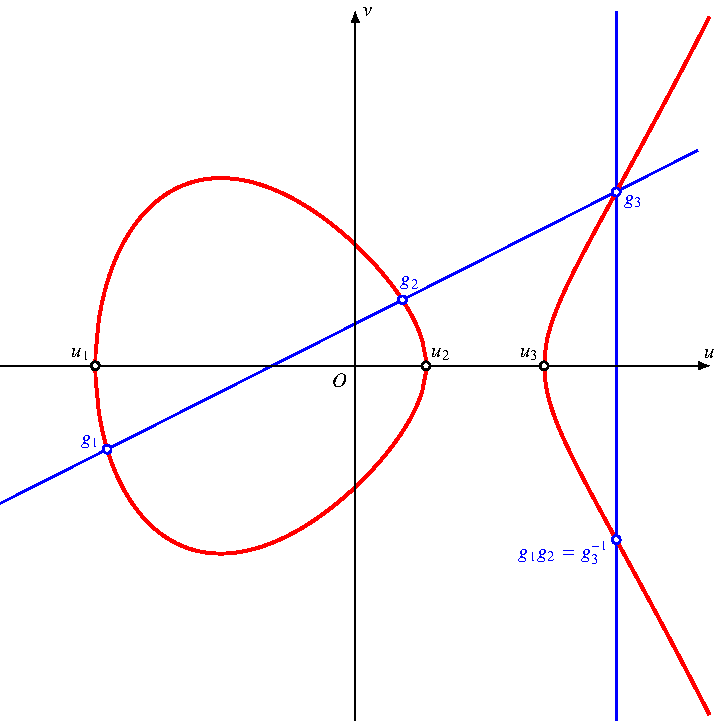
\includegraphics[width=\textwidth]{../../buch/chapters/90-crypto/images/elliptic.pdf}
\end{center}
\end{column}
\begin{column}{0.56\textwidth}
\uncover<3->{%
\begin{block}{Lösung}
Finde $h\in G$ derart, dass 
\begin{align*}
g(t)
&=
tg + (1-t)h
\\
\uncover<4->{%
\begin{pmatrix}X(t)\\Y(t)\end{pmatrix}
&=
t\begin{pmatrix}x_g\\y_g\end{pmatrix}
+(1-t) \begin{pmatrix}x_h\\y_h\end{pmatrix}
}
\end{align*}
\uncover<5->{eingesetzt
\[
p(t)
=
Y(t)^2+X(t)Y(t)-X(t)^3-aX(t)-b
=
0
\]}%
\uncover<6->{%
Nullstellen $0$ (doppelt) und $1$ hat:}
\[
\uncover<7->{p(t) = c(t^3-t)}
\]
\uncover<8->{Koeffizientenvergleich: einfachere Gleichungen für $x_h$ und $y_h$}
\end{block}}
\end{column}
\end{columns}
\end{frame}
\egroup
